\documentclass[a4paper,11pt]{article}
\usepackage{amsmath,amsthm,amsfonts,amssymb,amscd,amstext,vmargin,graphics,graphicx,tabularx,multicol} \usepackage[french]{babel}
\usepackage[utf8]{inputenc}  
\usepackage[T1]{fontenc} 
\usepackage[T1]{fontenc}
\usepackage{amsmath,amssymb}
\usepackage{pstricks-add,tikz,tkz-tab,variations}
\usepackage[autolanguage,np]{numprint} 
\usepackage{color}
\usepackage{ulem}

\setmarginsrb{1.5cm}{0.5cm}{1cm}{0.5cm}{0cm}{0cm}{0cm}{0cm} %Gauche, haut, droite, haut
\newcounter{numexo}
\newcommand{\exo}[1]{\stepcounter{numexo}\noindent{\bf Exercice~\thenumexo} : \marginpar{\hfill /#1}}
\reversemarginpar


\newcounter{enumtabi}
\newcounter{enumtaba}
\newcommand{\q}{\stepcounter{enumtabi} \theenumtabi)  }
\newcommand{\qa}{\stepcounter{enumtaba} (\alph{enumtaba}) }
\newcommand{\initq}{\setcounter{enumtabi}{0}}
\newcommand{\initqa}{\setcounter{enumtaba}{0}}

\newcommand{\be}{\begin{enumerate}}
\newcommand{\ee}{\end{enumerate}}
\newcommand{\bi}{\begin{itemize}}
\newcommand{\ei}{\end{itemize}}
\newcommand{\bp}{\begin{pspicture*}}
\newcommand{\ep}{\end{pspicture*}}
\newcommand{\bt}{\begin{tabular}}
\newcommand{\et}{\end{tabular}}
\renewcommand{\tabularxcolumn}[1]{>{\centering}m{#1}} %(colonne m{} centrée, au lieu de p par défault) 
\newcommand{\tnl}{\tabularnewline}

\newcommand{\trait}{\noindent \rule{\linewidth}{0.2mm}}
\newcommand{\hs}[1]{\hspace{#1}}
\newcommand{\vs}[1]{\vspace{#1}}

\newcommand{\N}{\mathbb{N}}
\newcommand{\Z}{\mathbb{Z}}
\newcommand{\R}{\mathbb{R}}
\newcommand{\C}{\mathbb{C}}
\newcommand{\Dcal}{\mathcal{D}}
\newcommand{\Ccal}{\mathcal{C}}
\newcommand{\mc}{\mathcal}

\newcommand{\vect}[1]{\overrightarrow{#1}}
\newcommand{\ds}{\displaystyle}
\newcommand{\eq}{\quad \Leftrightarrow \quad}
\newcommand{\vecti}{\vec{\imath}}
\newcommand{\vectj}{\vec{\jmath}}
\newcommand{\Oij}{(O;\vec{\imath}, \vec{\jmath})}
\newcommand{\OIJ}{(O;I,J)}

\newcommand{\bmul}[1]{\begin{multicols}{#1}}
\newcommand{\emul}{\end{multicols}}


\newcommand{\reponse}[1][1]{%
\multido{}{#1}{\makebox[\linewidth]{\rule[0pt]{0pt}{20pt}\dotfill}
}}

\newcommand{\titre}[5] 
% #1: titre #2: haut gauche #3: bas gauche #4: haut droite #5: bas droite
{
\noindent #2 \hfill #4 \\
#3 \hfill #5

\vspace{-1.6cm}

\begin{center}\rule{6cm}{0.5mm}\end{center}
\vspace{0.2cm}
\begin{center}{\large{\textbf{#1}}}\end{center}
\begin{center}\rule{6cm}{0.5mm}\end{center}
}



\begin{document}
\pagestyle{empty}
\titre{Contrôle 1 : Calcul numérique, Théorème de Pythagore et équations }{Nom}{Prénom}{Date}{Classe}

\begin{flushleft}
\begin{tabular}{|m{9.5cm}|m{1.25cm}|m{1.25cm}|m{1.25cm}|m{1.25cm}|m{1.25cm}|}
\hline 
\textbf{Compétences} & \begin{center}
\textbf{N.E.}
\end{center} & \begin{center}
\textbf{M.I.}
\end{center} & \begin{center}
\textbf{M.F.}
\end{center}  & \begin{center}
\textbf{M.S.}
\end{center} & \begin{center}
\textbf{T.B.M.}
\end{center} \\ 
\hline 
Je dois savoir traduire en langage mathématique une situation réelle \textit{(Exercice 2)} &  &  & & &\\
\hline 
Je dois savoir extraire d'un document les informations utiles, les reformuler, les organiser, les confronter à mes connaissances \textit{(Exercice 4)} &  &  & & &\\
\hline
Je dois savoir résoudre une équation du 1er degré à une inconnue \textit{(Exercice 1)} &  &  & & &\\
\hline
\end{tabular} 
\end{flushleft}

\textit{N.E = Non évalué ; M.I. = Maîtrise insuffisante ; M.F. = Maîtrise fragile ; M.S. = Maîtrise satisfaisante ; T.B.M. = Très bonne maîtrise}\\


\vspace*{0.25cm}




\exo{4} Résoudre les équations suivantes en détaillant vos réponses :

\bmul{4}

\qa $ x-10=45$\\

\columnbreak

\qa $ x+19=-65$\\

\columnbreak

\qa $11x=143$\\





\columnbreak

\qa $2x - 19 = 11 $\\




\emul

\vspace*{1cm}




\exo{4} Modéliser une situation.\\

 Pour la rentrée scolaire, Blandine achète 6 classeurs et un livre. Elle paie au total 27,60 euros. \\
 \textbf{Sachant que le prix du livre est 12 euros, quel est le prix d'un classeur ?}\\
 \textit{(Méthode : Choisir une inconnue, écrire une équation, la résoudre et répondre à la question.)}\\

\vspace*{1cm}

\exo{4} Modéliser une situation.\\

 Un père dispose de 1 600 euros pour ses trois enfants. Il veut que l'aîné ait 200 euros de plus que le second et
que le second ait 100 euros de plus que le dernier. \\
\textbf{ Comment fait-il cette répartition ? Combien ont d'argent chacun de ces 3 enfants ?}\\
 \textit{(Méthode : Choisir une inconnue, écrire une équation, la résoudre et répondre à la question.)}\\





\vspace*{1cm}

\exo{7} \\ Pour chacune des affirmations suivantes, dire si elle est vraie ou fausse. \textit{Chaque réponse doit être
justifiée.}\\

\q \textbf{Affirmation 1 :} "$\dfrac{2}{7}+\dfrac{9}{3}=\dfrac{2+9}{7+3}$"\\
\vspace*{0.25cm}

\q \textbf{Affirmation 2 :} "Le nombre -2 est une solution de l'équation suivante : $ 7x-5 = -19$."\\
\vspace*{0.25cm}


\q \textbf{Affirmation 3 :} "Le résultat du calcul $ \dfrac{3}{4}-\dfrac{9}{4} \times
\dfrac{1}{6}=$ est égal à $-\dfrac{1}{4} $."\\
\vspace*{0.25cm}


 






\newpage
\vspace*{0.5cm}

\exo{5} Un silo à grains permet de stocker des céréales. Un ascenseur permet d'acheminer le blé dans le silo.
L'ascenseur est soutenu par un pilier.\\


\includegraphics[scale=0.8]{pythagoresilo.eps} 

On modélise l'installation par la figure ci-dessous qui n’est pas réalisée à l’échelle :

\bmul{2}



\noindent - Les points C, E et M sont alignés.\\
- Les points C, F, H et P sont alignés.\\
- Les droites (MH) sont perpendiculaires à la droite (CH).\\
-  CH = 8,50 m et CF = 2,50 m.\\
- CE = 6,5 m et EF = 6 m.\\
- Hauteur du cylindre : HM = 20,40 m.\\




\columnbreak

\includegraphics[scale=0.7]{pythagoresilo2.eps} 



\emul

\initq \q  Quelle est la longueur CM de l’ascenseur à blé ?\\

\q L'ascenseur est soutenu par un pilier schématisé par le segment [EF] dans la figure. Ce pilier est-il bien perpendiculaire au sol ?\\
\vspace*{1cm}


\exo{+1,5} BONUS\\

Une brique
pèse
1
kg
plus
la
moitié
de
son
poids. \hspace*{1cm}
Combien
pèse-t-elle?


\end{document}
